Once the experiment was complete, a number of different results were extracted. It was important to know how the drone flew over the grid in comparison to the desired flight path. Considering that the drone flew across the grid and flew back across the grid in a different configuration, the forward and backward flight path of the drone was plotted across the desired flight path. Fig. (\ref{fig:FFP}) and Fig. (\ref{fig:BFP}) show the forward and backward flight path of the drone as well as the coverage area over which objects were placed. The red region in the figures indicates the area of interest. This region is smaller than the drone flight path to mitigate errors arising from the turning switchback sections of the flight path.
\begin{figure}[H]
  \centering
  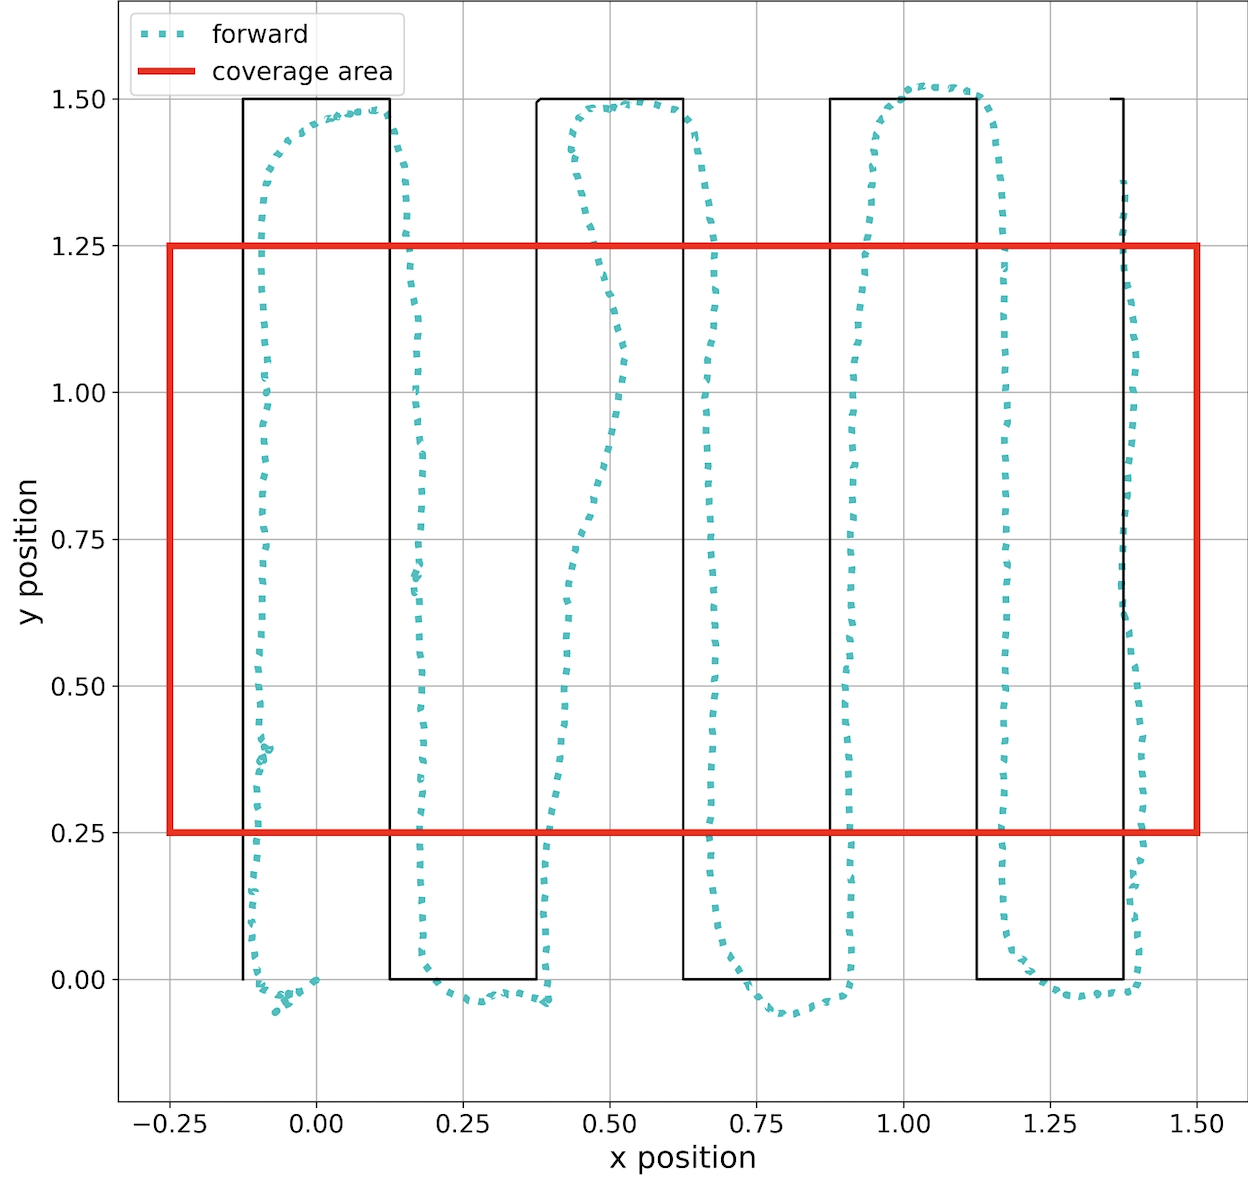
\includegraphics[width=0.7\linewidth, height=0.7\linewidth]{R&D/FFP.png}  
  \caption{Forward Flight Path}
  \label{fig:FFP}
\end{figure}

From Fig. (\ref{fig:FFP}) it is clear that the drone flew pretty close to the desired flight path going forward (left to right) across the grid. The red lined box represents the area in which objects were placed to provide the drone more time to stabilize once it cleared the object filled regions. Objects weren't placed all over the area of coverage, just in certain regions, to provide a more realistic grid to map out. We see at points in time where it deviates from the desired flight path, and the reason for this was that an object was placed there, and whenever the drone sensed the edge of an object, it increased the z-position that it was flying at, and that sudden increases caused it to lose control and stability a little bit, resulting in the drone not flying on the desired flight path. Whenever the drone was flying over the center of an object, it is seen that the drone did not deviate as much from the desired flight path. Between 0.375 m and 0.5 m in the x position, the drone is seen to deviate the most, and this was a result of the edge of an object being located there, which was a challenge faced using just the flow deck. Complex configurations of objects could not be flown over without deviation, which is where the loco-positioning system would have provided more accurate results. Regardless of these deviations, as shown in Fig. (\ref{fig:PvsT}), the actual flight path of the drone was not far from the desired flight path of the drone in terms of its x and y position. 

\begin{figure}[H]
  \centering
  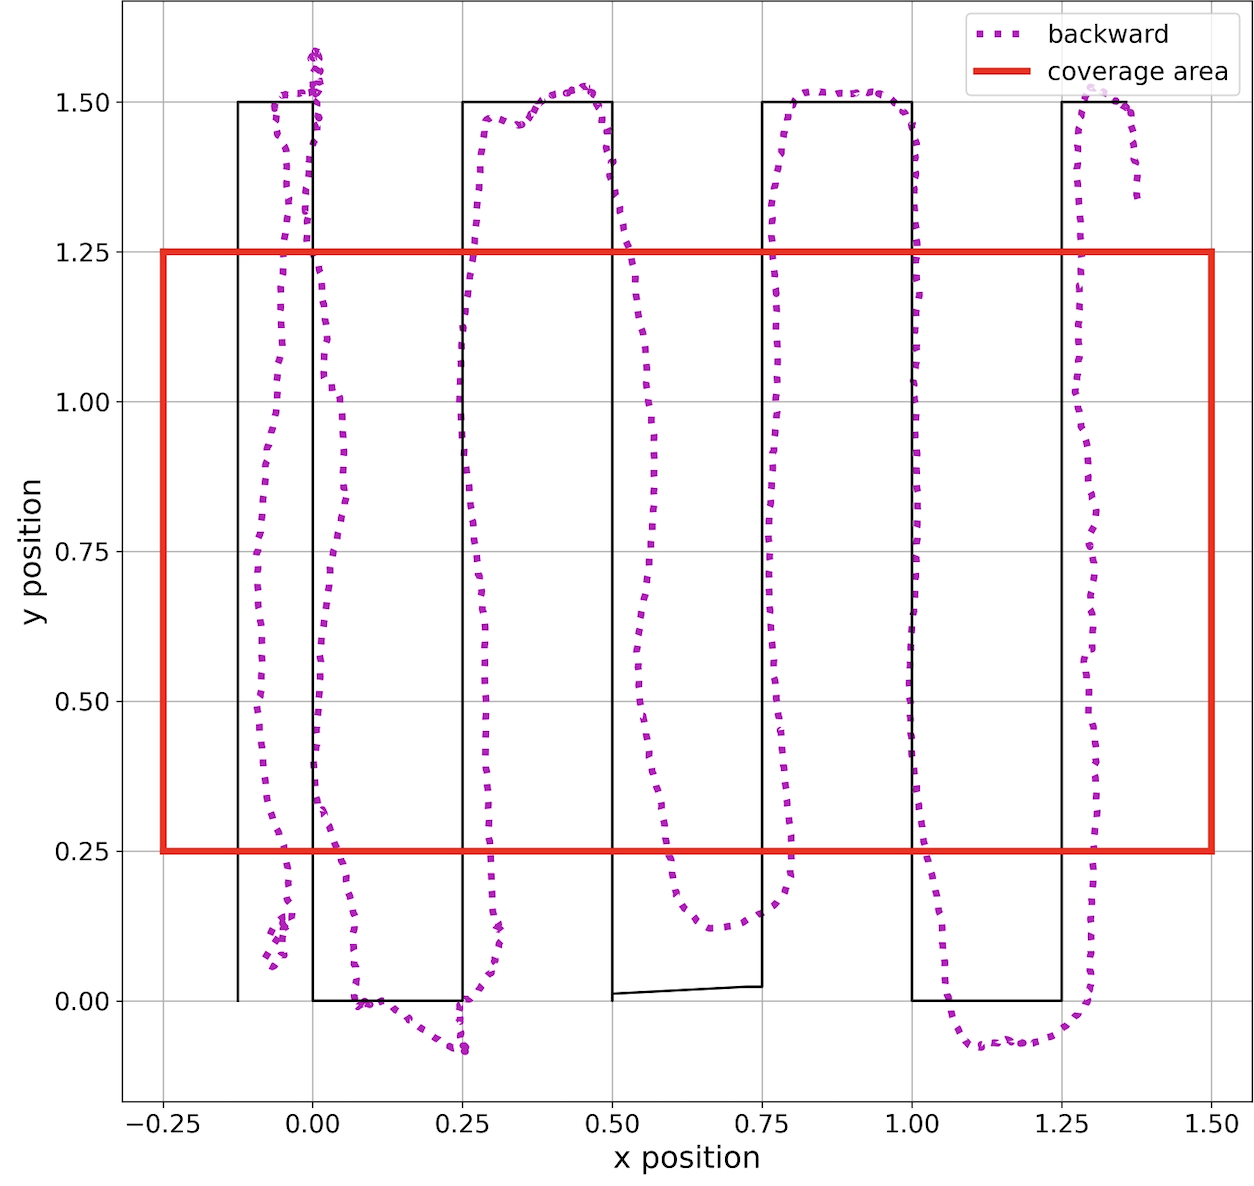
\includegraphics[width=0.7\linewidth, height=0.7\linewidth]{R&D/BFP.png}  
  \caption{Backward Flight Path}
  \label{fig:BFP}
\end{figure}

Fig. (\ref{fig:BFP}) shows the backward flight path (right to left) of the drone, to go from a location of (1.5 m, 1.5 m) in the (x,y) position back to origin, located at (0,0). The initial movement to turn back around to fly back to origin was a sharper turn than normal ones, with a distance of only 0.125 m. The drone is seen to follow a the desired flight path pretty accurately for the first couple turns, but at around a similar position as seen in Fig. (\ref{fig:FFP}), the drone is seen to deviate from the desired flight path as it hits the edge of an object. Similarly, near the end of the flight of the drone, we see the drone going a little haywire, and losing control as it hits the edge of another object - a result of a modified flight path. During forward motion, the drone flew over the center of the object, which caused it to remain stable, but on the way back, it sensed the edges, which is something that the group wanted to test out; the reaction of the drone flying over the edges of the object. This resulted in the drone taking a lot longer to stabilize considering the drone didn't sense it with the entire camera because of the camera's FOV, and that resulted in the drone moving in the North-west direction in the z-axis rather than just north. Therefore, from both the forward and backward flight path graphs, it is evident that the drone worked best when its camera's FOV was only sensing a completely flat surface rather than different altitude surfaces. To ensure that the path of the drone in both the x and y direction was identical or similar to the provided inputs, a plot of the x and y position of the drone was plotted against its desired x and y position.

\begin{figure}[H]
  \centering
  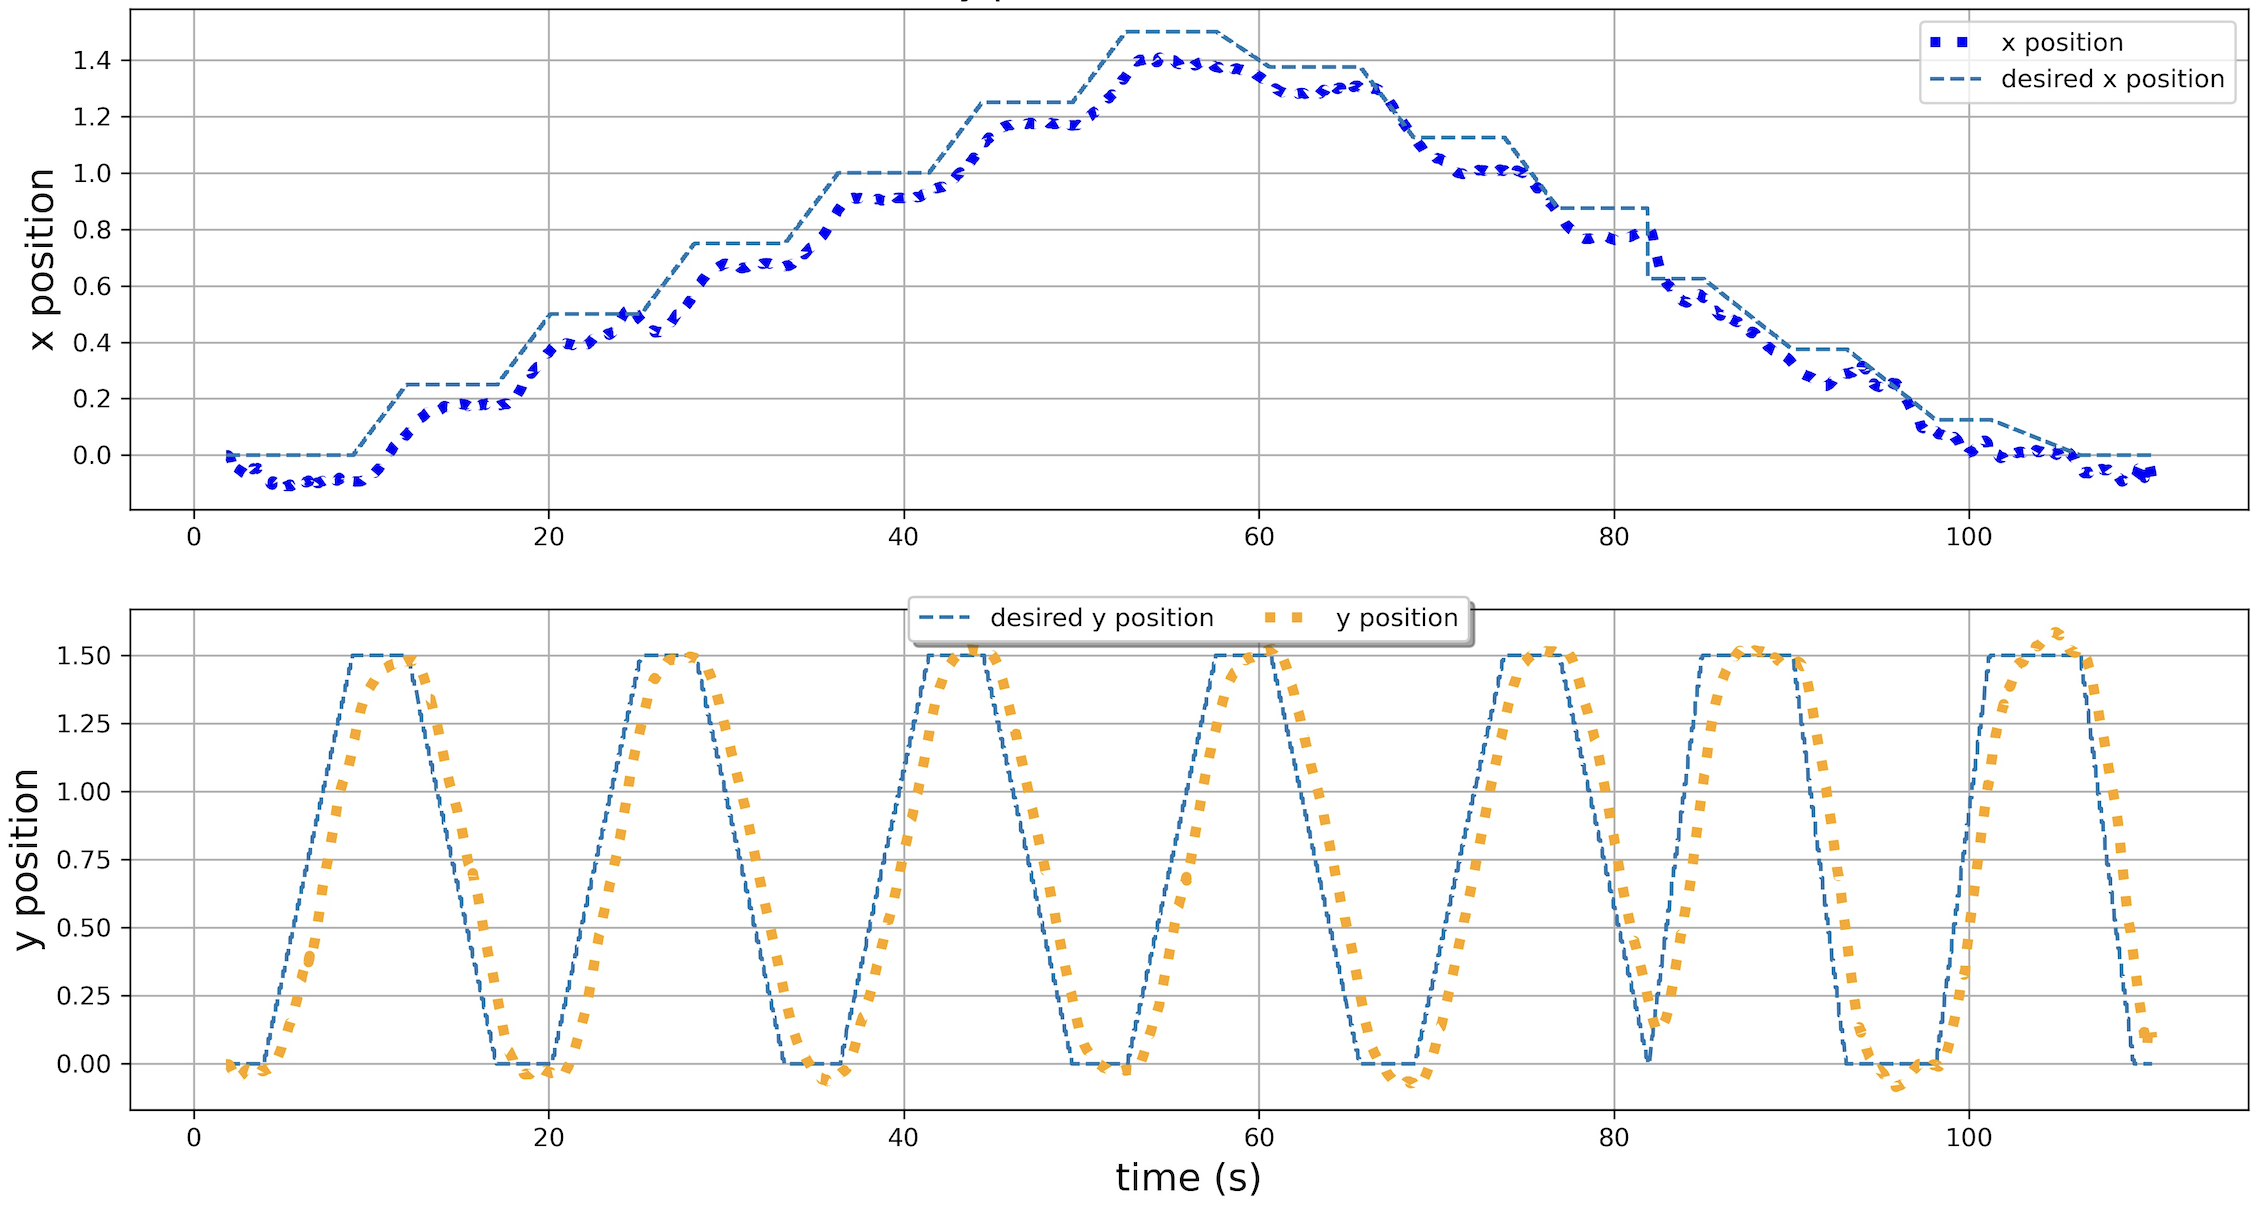
\includegraphics[width=0.8\linewidth, height=0.6\linewidth]{R&D/PvsT.png}  
  \caption{X and Y Position vs. Time}
  \label{fig:PvsT}
\end{figure}

Fig. (\ref{fig:PvsT}) shows the x and y position of the drone and the desired x and y position of the drove against time. The total flight time for the drone to complete the entire forward and backward flight path was about 112 seconds. Our initial tests completed the entire flight in a much shorter period of time, but the trade off was that the drone was not as stable, and was not tracking the desired positions as accurately as our final test. As the graph shows, at a slower speed, the drone was able to fly over the object filled grid more accurately with a slight offset in the x position (in a negative manner), and a slight offset in the y position in terms of at what time it went over the desired y positions. From the x-position graph, we can see that at the start, the drone sweep-ed a little bit when taking off, causing it to go into the negatives of the x-position, which is why throughout the flight test, it was about 0.05 m off the desired x-position. From the y-position graph, we can see that at the start, there was also a delay in terms off the drone taking off, resulting in it being offset to the desired y position by about 1.5 seconds. There are some larger deviations seen in the graph from the desired position, where the graph is not following the trend of the desired x and y position, and these occurred when the drone flew over an edge of an object, and this was an expected result for the team. When implementing the project using just the flow deck, there was a trade-off between using the loco-positioning system and just the flow deck, and that was based off of the complexity of objects that the drone would be able to successfully fly over to create a topographical map. Overall, the graphs show that the drone was able to fly across the grid close to the desired positions provided to the drone. The RMSE values of the drone flight over the empty grid and the object filled grid are given in the tables below.

\begin{center}
\captionof{table}{\textbf{RMSE Values of Drone Flight with Targets for Empty Grid}}

    \begin{tabular}{|c|c|c|}
        \rowcolor{lightgray} 
        \hline
        \textbf{State} & \textbf{Experimental RMSE} & \textbf{Target RMSE} \\
        \hline
        o_x & 0.0134 & 0.075 \\
        \hline
        o_y & 0.190 &  0.075  \\
        \hline
        o_z & 0.016 &  0.075  \\
        \hline
        \psi & 0.011 &  0.050  \\
        \hline
        \theta & 0.014 &  0.015 \\
        \hline
        \phi & 0.014 &  0.015 \\
        \hline
\end{tabular}
\end{center}

\begin{center}
\captionof{table}{\textbf{RMSE Values of Drone Flight with Targets for Object Filled Grid}}

    \begin{tabular}{|c|c|c|}
        \rowcolor{lightgray} 
        \hline
        \textbf{State} & \textbf{Experimental RMSE} & \textbf{Target RMSE} \\
        \hline
        o_x & 0.095 & 0.075 \\
        \hline
        o_y & 0.229 &  0.075 \\
        \hline
        o_z & 0.479 &  0.075 \\
        \hline
        \psi & 0.011 &  0.050 \\
        \hline
        \theta & 0.014 &  0.015 \\
        \hline
        \phi & 0.014 &  0.015 \\
        \hline
\end{tabular}
\end{center}

\begin{figure}[H]
\centering
\begin{subfigure}{0.9\textwidth}
  \centering
  % include First image
  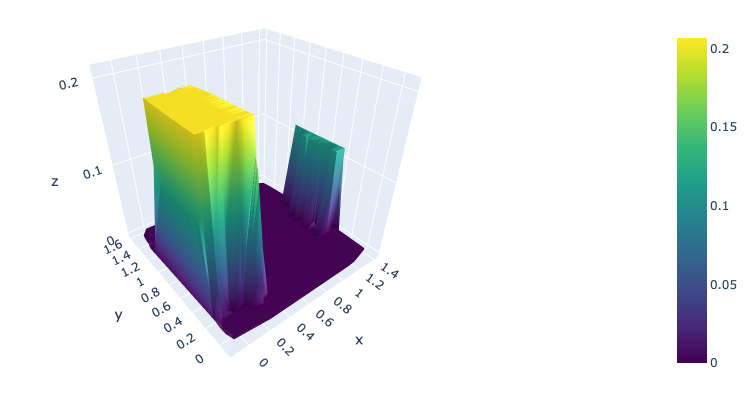
\includegraphics[width=0.85\linewidth]{R&D/3Dplot1.png}
  \caption{View 1}
  \label{fig:F3DP}
\end{subfigure}
\begin{subfigure}{0.9\textwidth}
  \centering
  % include Second image
  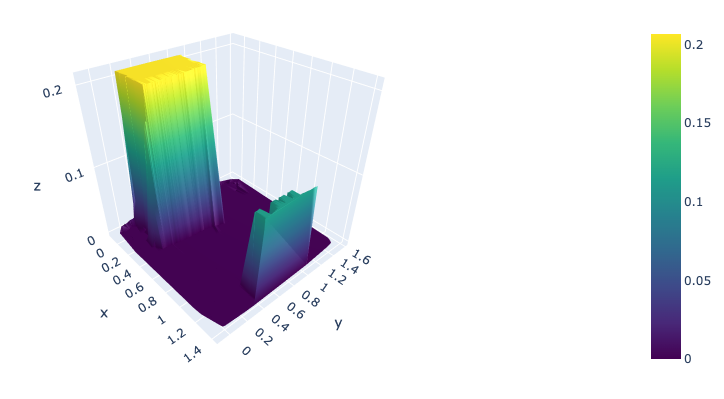
\includegraphics[width=0.85\linewidth]{R&D/3Dplot2.png}
  \caption{View 2}
  \label{fig:B3DP}
\end{subfigure}
\caption{Post-Processed Topographical Visualization of the location the Drone Flew Over}
\label{fig:3DP}
\end{figure}

Fig. (\ref{fig:3DP}) shows a successful visualization of the object filled grid. Both the forward and backward flight were used to create a post-processed topographical visualization of the grid. Objects were placed as shown in Fig. (\ref{fig:OFG}), and from Fig. (\ref{fig:F3DP}) and Fig. (\ref{fig:B3DP}) the approximate (x,y,z) positions of the objects can be seen. 

Post processing was done by first getting the (x,y) locations of the first and last peaks in the flight path for each object as shown in the figure \ref{fig:r1}. From these locations, and because it was known that the objects were rectangular, the area of the objects could be determined. It is necessary to note that due to not using the loco-positioning deck, the unobservability of the x and y positions cause significant drift in the x and y directions. The actual and experimentally determined x and y dimensions of the objects are given in the table below. With more testing correction factors could be developed to mitigate the error in these measurements if the loco-positioning deck is not used. From the current testing done a correction factor of $75\%-80\%$ could be employed to get the proper (x,y) dimensions of the objects.

\begin{center}
\captionof{table}{\textbf{Brown Box Dimensions}}

    \begin{tabular}{|c|c|c|}
        \rowcolor{lightgray} 
        \hline
        \textbf{Actual [cm]} & \textbf{Experimental [cm]} & \textbf{Percent Error [\%]} \\
        \hline
        x = 16.5 & x = 29 & 75.76 \\
        \hline
        y = 38 & y = 68 &  78.95 \\
        \hline
\end{tabular}
\end{center}

\begin{center}
\captionof{table}{\textbf{Black Box Dimensions}}

    \begin{tabular}{|c|c|c|}
        \rowcolor{lightgray} 
        \hline
        \textbf{Actual [cm]} & \textbf{Experimental [cm]} & \textbf{Percent Error [\%]} \\
        \hline
        x = 10 & x = 18 & 80.00 \\
        \hline
        y = 24.5 & y = 44 & 79.59\\
        \hline
\end{tabular}
\end{center}

\begin{figure}[H]
  \centering
  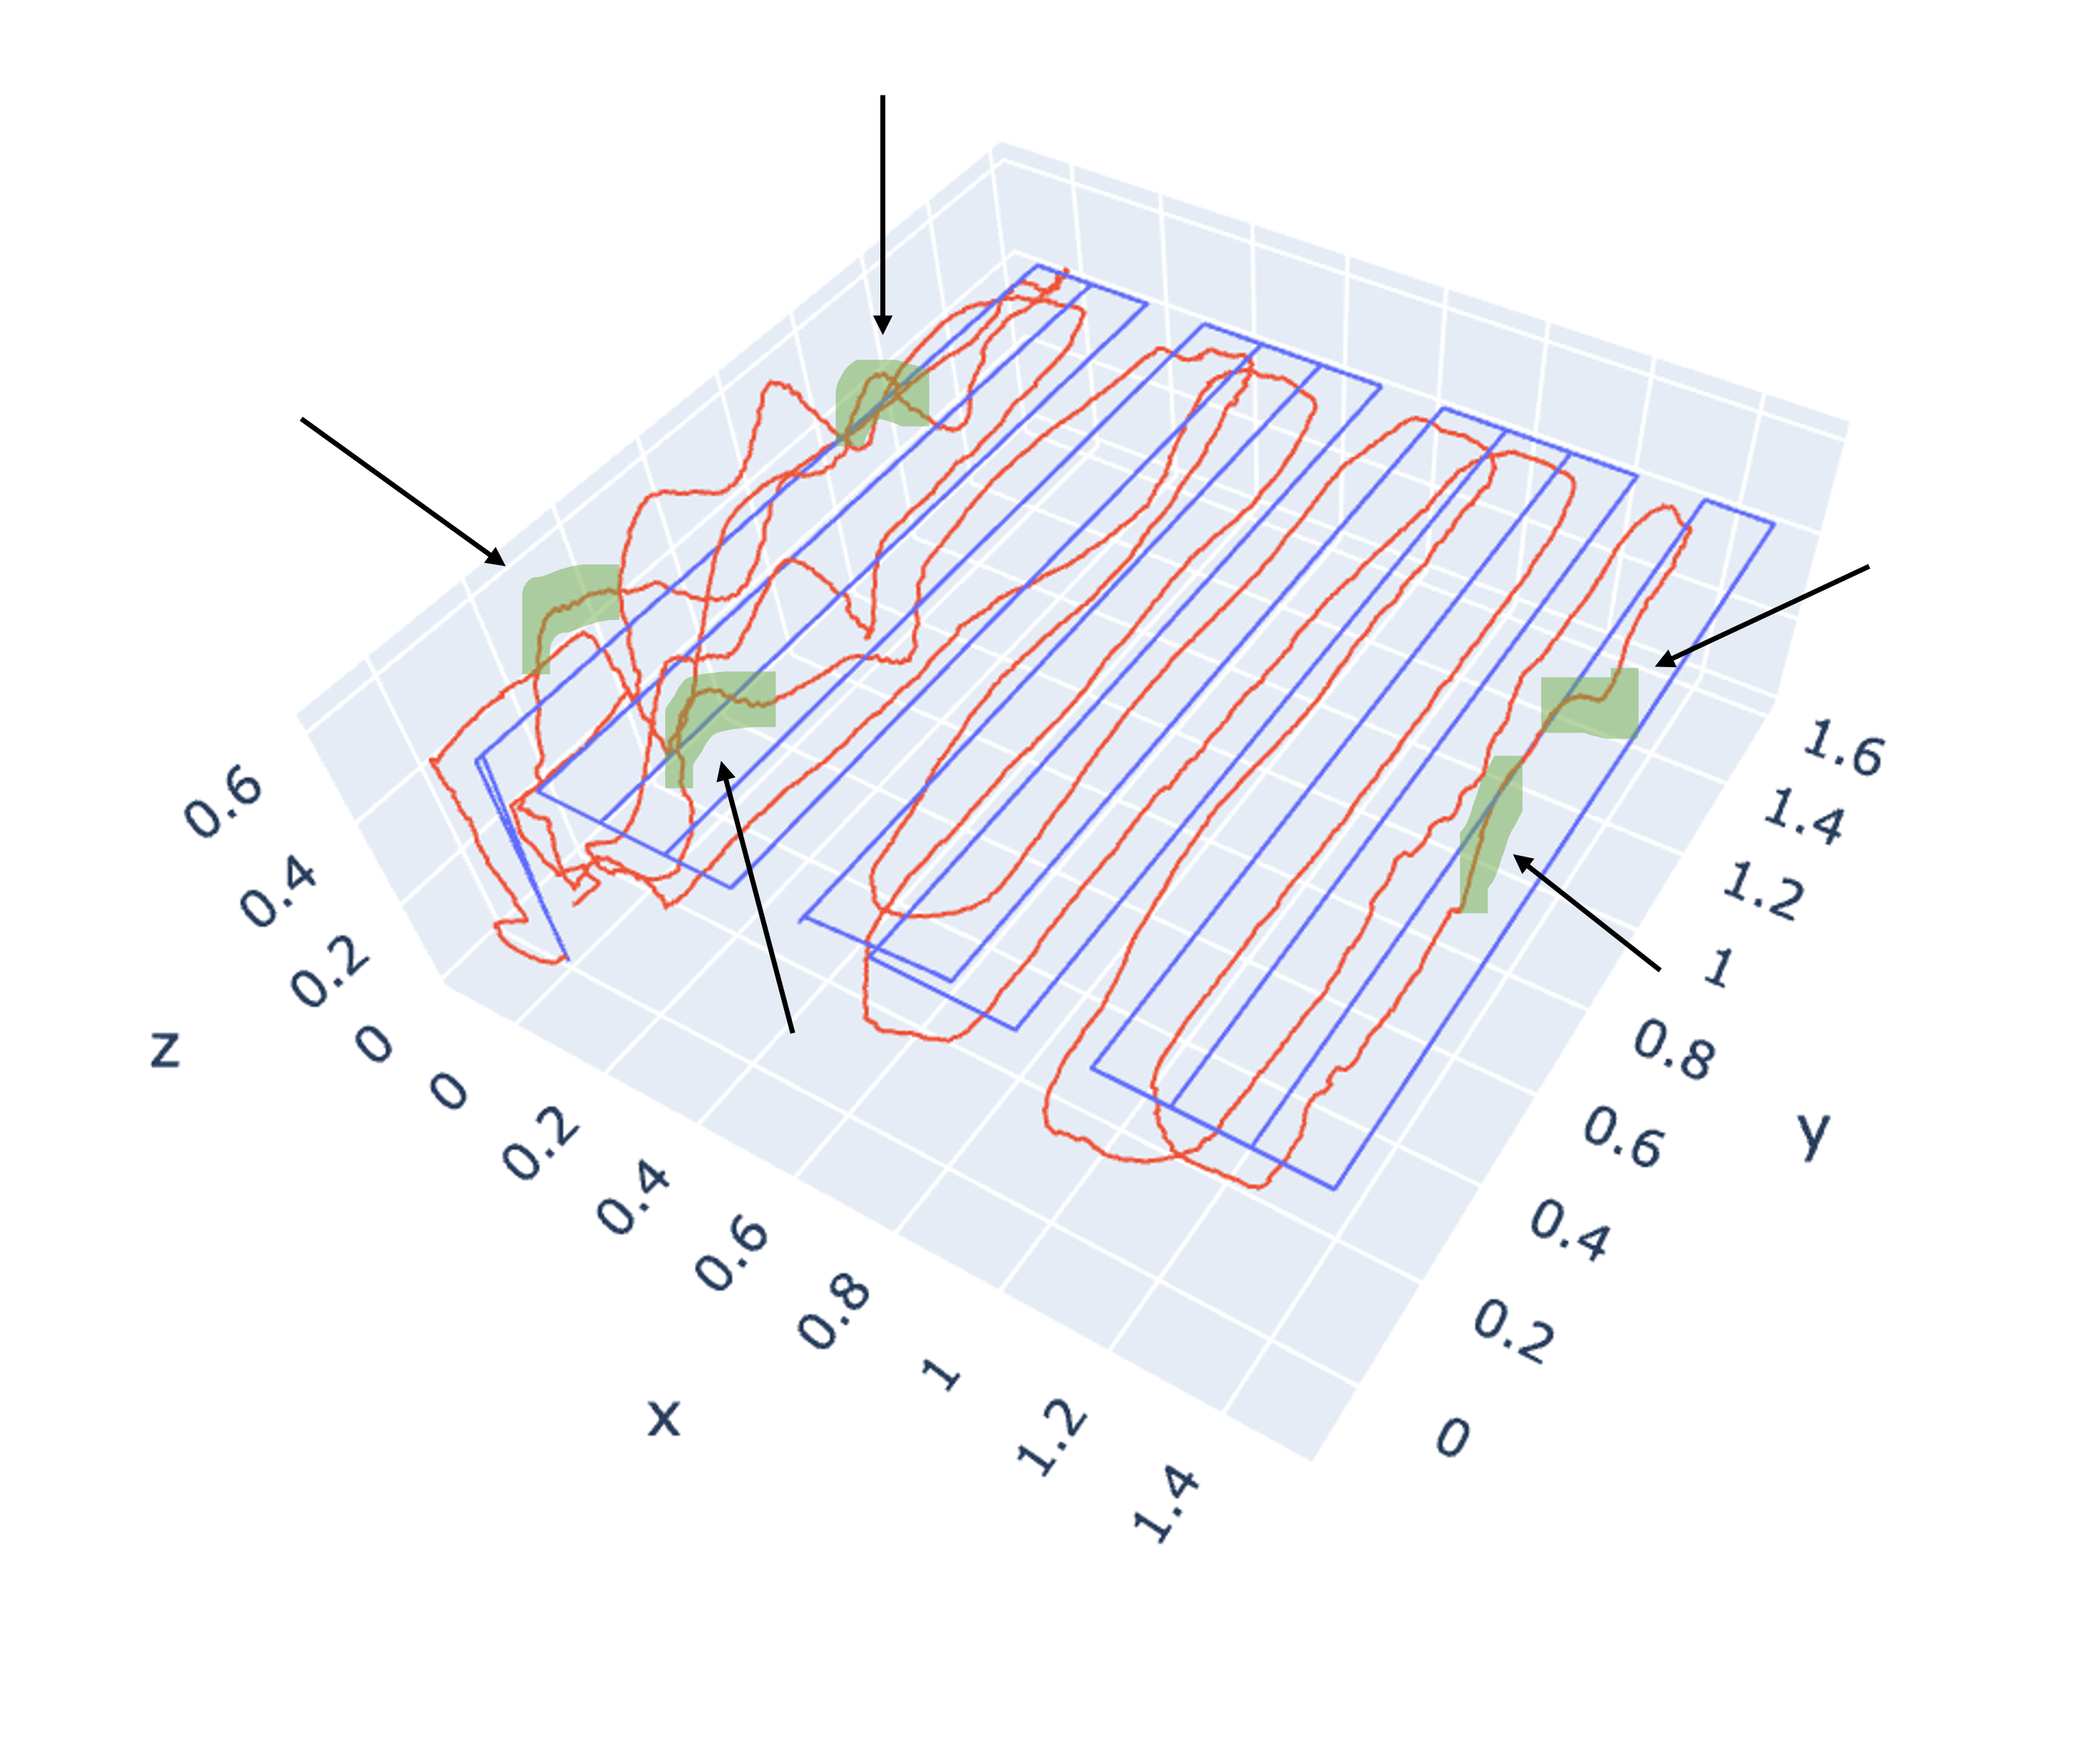
\includegraphics[width=0.8\linewidth]{R&D/r1.png}  
  \caption{Peaks in 3D Flight Path for (x,y) Approximate Position Extraction}
  \label{fig:r1}
\end{figure}

The z-direction measurements are much more accurate due to the observability of the state. For conciseness the process for determining the height of the brown box is detailed below; the procedure for the black box is identical. The z-position was extracted by subtracting the peak heights, indicated by the orange arrows, from the subsequent hover heights, indicated by the yellow highlight in the figure \ref{fig:r2}. The hover heights were average over a slice of time as the drone did not hover at exactly 0.45 m. After averaging all of the values from each peak and hover pair, the final height of the brown box was determined to be $0.1732$ meters. When compared with the actual object height of $0.2050$ meters, the margin of error was $15.51\%$. Following a similar procedure for the black box, the experimentally determined height was $0.0848$ meters, the actual height was $0.12$ meters, and the margin of error was $5.67\%$. A correction factor was applied by averaging the difference between the experimental and actual values for both objects. After the correction factor, which was $0.0335$, was applied the new z-positions were $0.2067$ and $0.1183$ with margins of error $0.83 \%$ and $1.42 \%$. All of this data has been tabulated below.

\begin{center}
\captionof{table}{\textbf{Object Heights}}

    \begin{tabular}{|c|c|c|c|}
        \rowcolor{lightgray} 
        \hline
        \textbf{Object} & \textbf{Actual [cm]} & \textbf{Experimental [cm]} & \textbf{Percent Error [\%]} \\
        \hline
        Brown Box & z = 17.32 & z = 20.50 & 15.51\%\\
        \hline
        Black Box & z = 8.48 & z= 12.00 &5.67\% \\
        \hline
\end{tabular}
\end{center}

\begin{center}
\captionof{table}{\textbf{Object Heights After Correction}}

    \begin{tabular}{|c|c|c|c|}
        \rowcolor{lightgray} 
        \hline
        \textbf{Object} & \textbf{Actual [cm]} & \textbf{Experimental [cm]} & \textbf{Percent Error [\%]} \\
        \hline
        Brown Box & z = 20.67 & z = 20.50 & 0.83\%\\
        \hline
        Black Box & z = 11.83 & z= 12.00 & 1.42\% \\
        \hline
\end{tabular}
\end{center}

\begin{figure}[H]
  \centering
  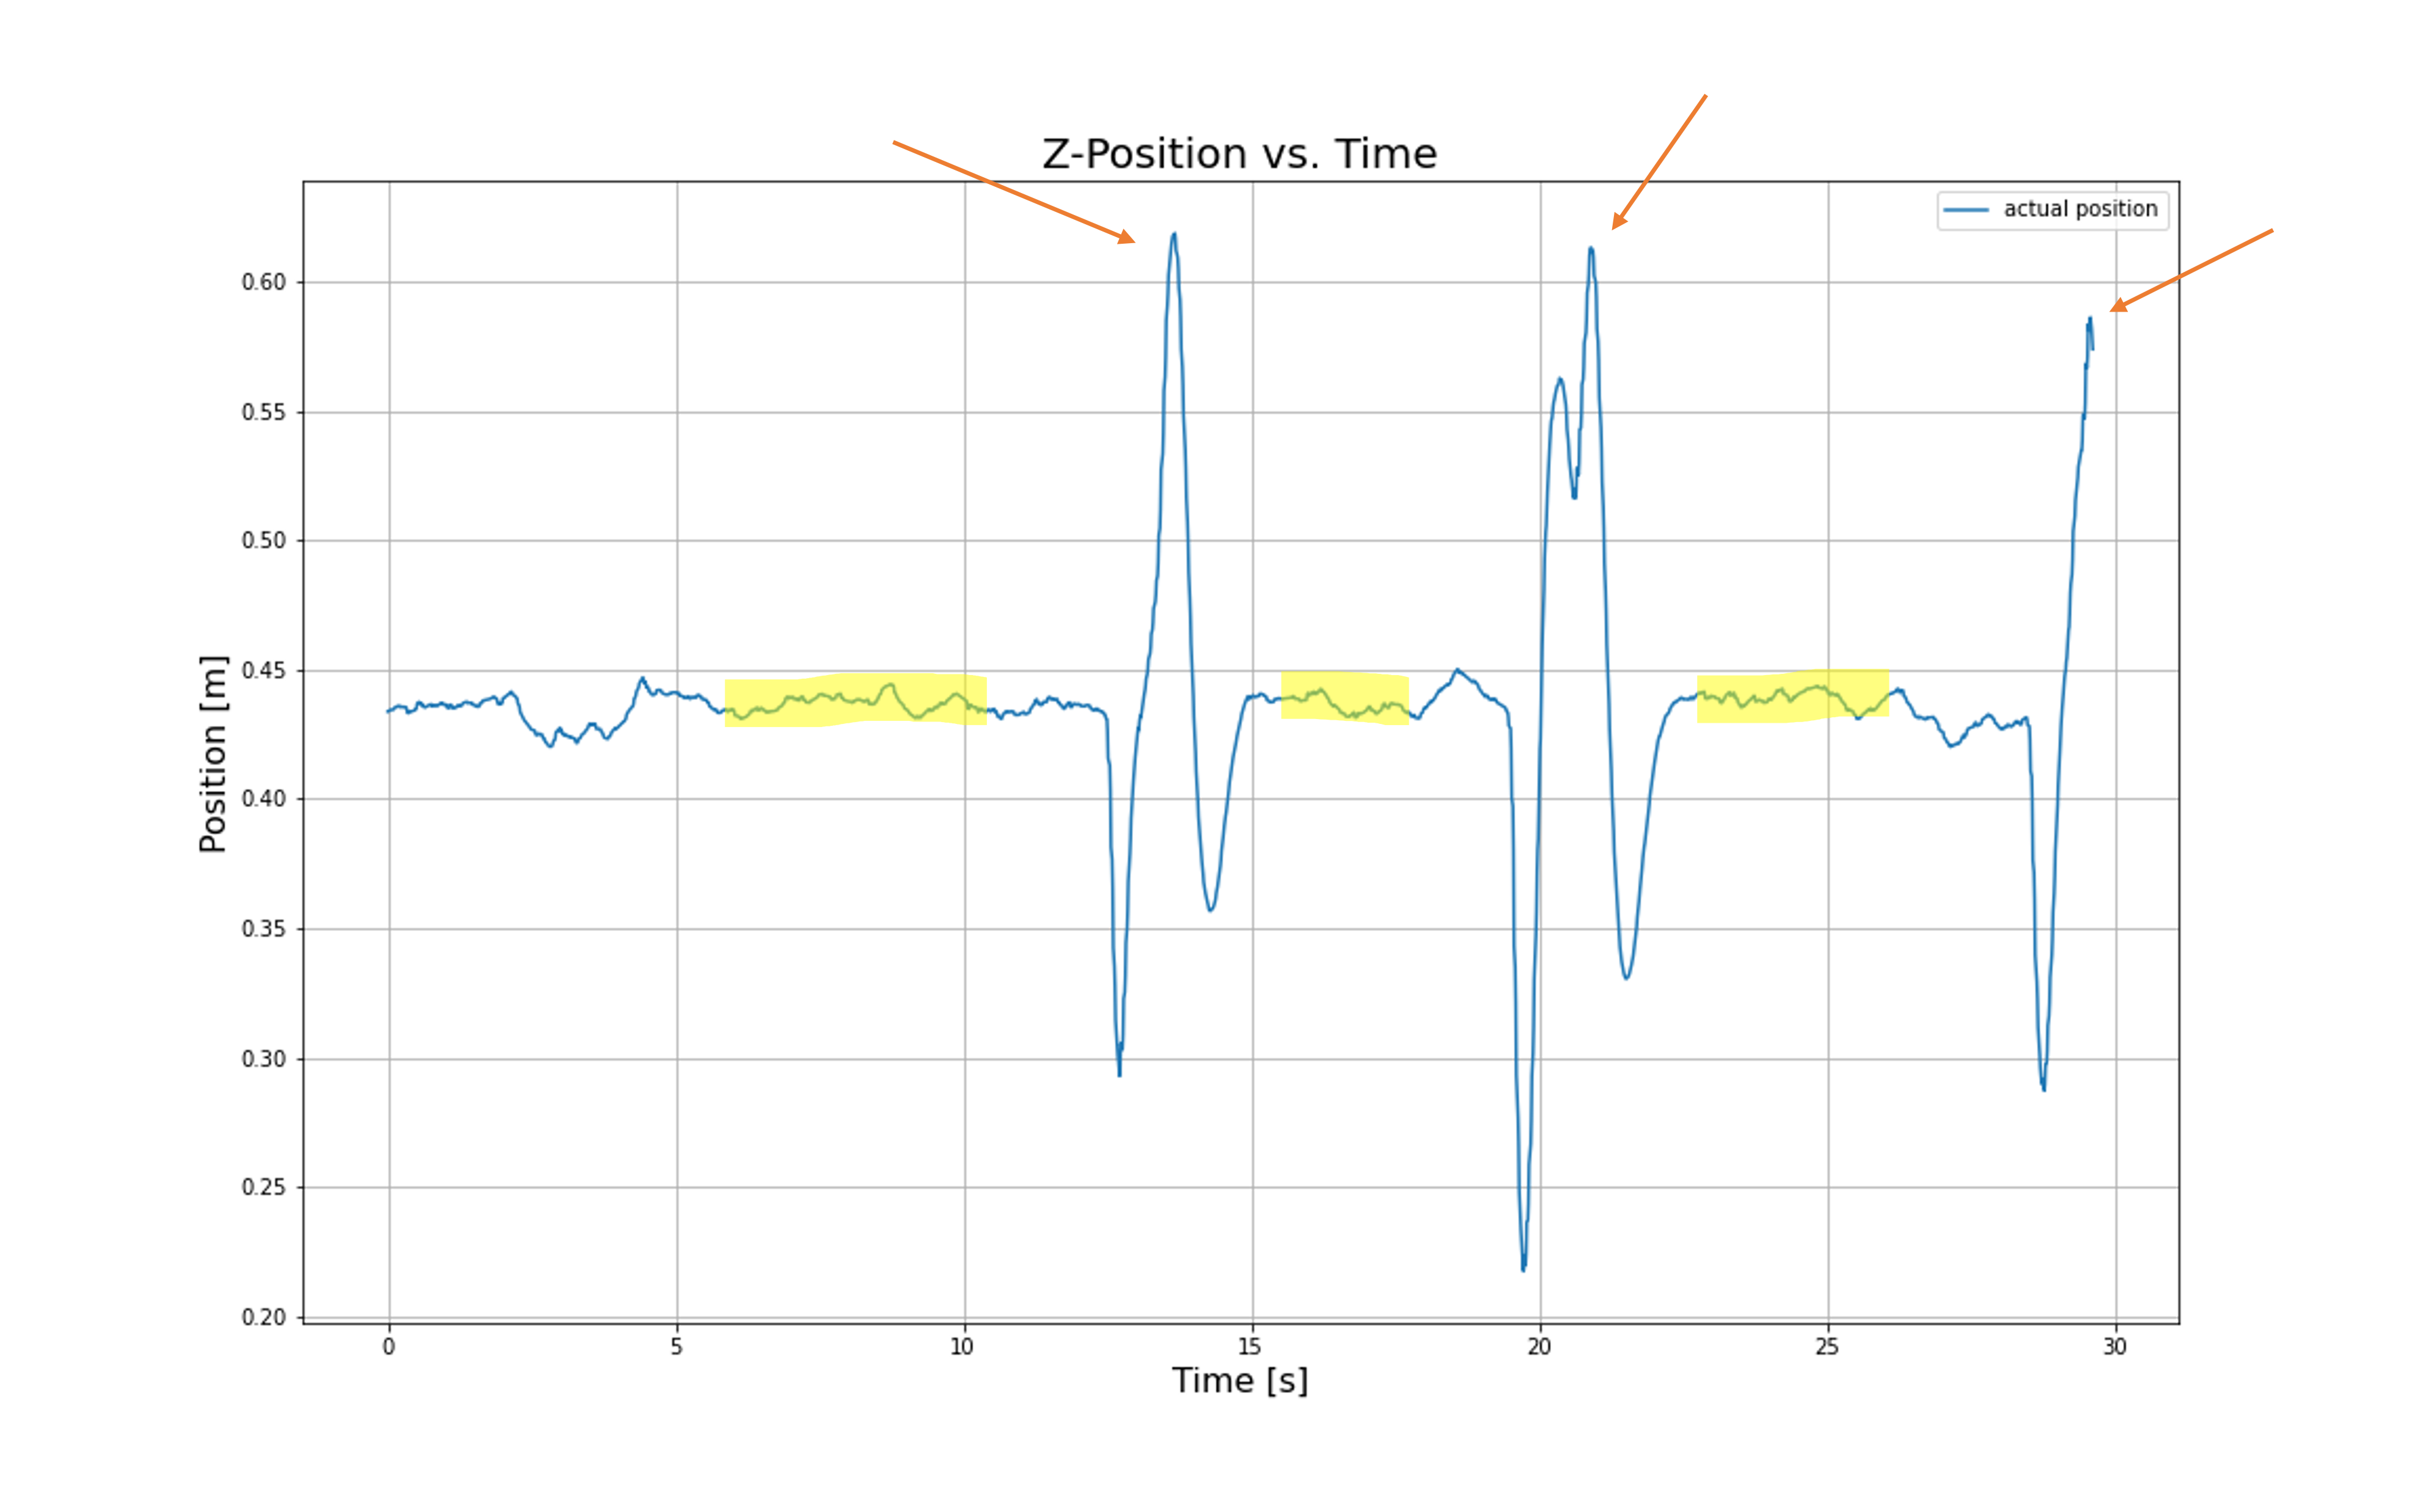
\includegraphics[width=1.0\linewidth]{R&D/r2.png}  
  \caption{Peaks in Z-Position vs. Time for Z-Position Extraction}
  \label{fig:r2}
\end{figure}

Once all of the positional information was determined the plot was smoothed out by subtracted the flight altitude from the z-positional data. This was done to make the floor of the test section coincide with the "floor" in the map. Then from the range of (x,y) values the z-positional data was modified to be that of the corrected object heights respectively. This resulted in the final plots shown above. Overall, the graphs that were visualized were accurate and provided a pretty good representation of the grid that the drone was flying over. The area the objects cover is larger than in actuality, however the true object locations are encompassed by this area. In addition this can be corrected by using a correction factor or loco-positioning deck as discussed. The group was able to show that the drones basic flow deck could be implemented when mapping out various different surfaces to provide a good approximation of what the surface in question would look like.
